\documentclass[a4paper,fleqn]{cas-sc}

\usepackage[authoryear,longnamesfirst]{natbib}
\usepackage{amsmath,amssymb}
\usepackage{booktabs}
\usepackage{graphicx}
\usepackage{multirow}
\usepackage{threeparttable}
\usepackage{xurl}
\usepackage{xcolor}
\usepackage{tabularx}
\usepackage{enumitem}
\usepackage{float}
\usepackage{placeins}

% Verified author and repository details supplied/audited on 5 September 2026.
% Repository values are mirrored in data_code_availability.txt.
\newcommand{\AuthorName}{Vahid Solouk}
\newcommand{\AuthorShortName}{Solouk}
\newcommand{\AuthorTitle}{Associate Professor}
\newcommand{\AuthorEmail}{v.solouk@it.uut.ac.ir}
\newcommand{\AuthorORCID}{0000-0001-8304-6394}
\newcommand{\AuthorProfileURL}{}
\newcommand{\AffiliationOrganization}{Urmia University of Technology}
\newcommand{\AffiliationAddress}{Department of IT and Computer Engineering, Off Jaame-Jam HW}
\newcommand{\AffiliationCity}{Urmia}
\newcommand{\AffiliationPostcode}{57166}
\newcommand{\AffiliationCountry}{Iran}
\newcommand{\RepositoryURL}{https://github.com/vsolouk-cmyk/xauusd-trader}
\newcommand{\RepositoryCommit}{0c24c7a47b36642e675a4de1b2f5829a40195666}
\newcommand{\FundingStatement}{This research received no specific grant from any funding agency in the public, commercial, or not-for-profit sectors.}
\newcommand{\InterestStatement}{The author declares that there are no known competing financial interests or personal relationships that could have appeared to influence the work reported in this paper.}


\newcommand{\bps}{\,\text{bps}}
\newcommand{\xau}{\text{XAUUSD}}

\begin{document}
\let\WriteBookmarks\relax
\def\floatpagepagefraction{.8}
\def\textpagefraction{.1}

\shorttitle{From Apparent Edge to No-Go}
\shortauthors{\AuthorShortName}

\title[mode=title]{From Apparent Edge to No-Go: A Point-in-Time, Cost-Aware Audit of Heterogeneous XAUUSD Trading Strategies}

\author[1]{\AuthorName}[orcid=\AuthorORCID]
\cormark[1]
\credit{Conceptualization, Methodology, Software, Validation, Formal analysis, Investigation, Data curation, Writing -- original draft, Writing -- review and editing, Visualization, Project administration}

\affiliation[1]{organization={\AffiliationOrganization},
  addressline={\AffiliationAddress},
  city={\AffiliationCity},
  postcode={\AffiliationPostcode},
  country={\AffiliationCountry}}

\cortext[1]{Corresponding author: \AuthorEmail.}

\begin{abstract}
Backtested trading strategies are often evaluated after extensive specification search, creating a risk that apparently attractive returns reflect omitted costs, selection effects, unstable samples, or feed-specific signals. This study conducts a retrospective, point-in-time audit of a heterogeneous XAUUSD research program through a prospectively locked consolidated rerun. The registry contains 47 specifications. Thirty-nine primary specifications spanning 20 economic families were recomputed; eight machine-learning combinations were retained as forensic records and excluded from primary inference. The run used source-native severe costs, prohibited historical strategy-result files as computational inputs, and computed no post-2024 outcomes. Familywise evidence was evaluated with a centered circular moving-block max-$t$ bootstrap and supplemented by source-native acceptance gates, deflated Sharpe ratios, a pre-declared timestamp-alignment sensitivity test, and cross-feed replication where applicable. The 39 specifications generated 28,685 normalized trade or rebalance records. Positive means declined from 24 specifications before costs to 9 under normal costs, 5 under severe costs, and 1 under a common fixed-stress schedule. No specification passed its complete native gate set, and none of the 20 families was supported. The minimum familywise adjusted $p$-value was 0.446, and the maximum deflated-Sharpe probability was 0.011. Seven of 20 cross-feed-eligible specifications failed replication, including two sign reversals. The evidence does not rule out every possible gold-market effect. It shows that apparent profitability within the locked universe did not survive the joint economic, statistical, temporal, and data-source requirements needed for a defensible trading-edge claim.
\end{abstract}

\begin{highlights}
\item Positive strategy means fell from 24 gross to 5 after severe costs.
\item No specification passed its complete source-native acceptance gates.
\item No family survived a 20-day block max-$t$ multiplicity correction.
\item Seven of 20 eligible specifications failed cross-feed replication.
\item The audit retains complete negative evidence under a locked protocol.
\end{highlights}

\begin{keywords}
Gold \sep XAUUSD \sep technical trading \sep data snooping \sep transaction costs \sep multiple testing \sep reproducible finance
\end{keywords}

\maketitle

\section{Introduction}\label{sec:introduction}

Empirical trading research faces a structural asymmetry. A profitable rule can be discovered by trying many signals, parameters, horizons, filters, data transformations, and execution conventions, yet the final report usually presents only a small fraction of that search. The reported return is therefore evaluated against the visible specification, whereas its evidential burden is determined by the much larger research process that produced it. Reusing the same historical record for discovery and inference makes apparently satisfactory results possible even when none of the candidate mechanisms has genuine predictive content \citep{white2000,sullivan1999}. Transaction costs compound this problem. Rules selected on gross performance are often precisely those that trade most aggressively, so an ex post cost deduction can change both economic rankings and the identity of the apparent winner \citep{bajgrowicz2012}.

These concerns are especially important for gold trading. Gold is simultaneously a commodity, a monetary asset, a dollar-denominated international security, and a candidate hedge or safe haven \citep{baur2010hedge,baur2010safe}. Recent evidence reinforces the point that these roles are state-, horizon-, and market-dependent rather than fixed attributes \citep{gurdgiev2024,ryan2024,faraj2025,xu2026}. Gold prices can therefore respond to exchange rates, interest rates, inflation, risk sentiment, policy uncertainty, and conditions in related commodity markets. This economic richness supports many plausible trading hypotheses, but it also creates many degrees of freedom. A gold strategy may be expressed as a price-only technical rule, a response to macroeconomic events, a cross-asset threshold, a long-horizon trend rule, or a relative-value position against silver. Evaluating one selected rule in isolation can conceal the effective multiplicity created by the research program around it.

The empirical record on technical trading illustrates the difficulty. Early work documented non-random return patterns under familiar moving-average and range rules \citep{brock1992}. Later research emphasized data-snooping-robust tests, trading costs, persistence, and genuine out-of-sample evaluation \citep{hsu2010,bajgrowicz2012}. Recent large-universe studies have not resolved the debate; they have made its conditional nature clearer. Evidence differs across currencies, equities, and spreads, changes across subperiods, and can deteriorate after costs or out of sample \citep{dockery2023,psaradellis2023,rink2023,song2025}. In precious metals specifically, \citet{batten2018} find that standard intraday technical parameters have no predictive power, while some broader gold parameter combinations appear significant; \citet{jin2022}, after accounting for data snooping, costs, market conditions, and rebalancing frequency, concludes that persistent attractive out-of-sample performance in China's gold futures market is unlikely. The relevant question is consequently not whether one backtest is positive, but whether the candidate remains credible once the search process, implementation economics, temporal behavior, and measurement source are exposed.

This paper studies that chain in a heterogeneous XAUUSD research program. The project had examined many historical outcomes before the present study was designed. It would therefore be inaccurate to label the whole project a prospective experiment or to treat its final registry as if it had been created without knowledge of the data. Instead, the design is a retrospective systematic audit followed by a prospectively locked \emph{consolidated rerun}. Before that rerun, 47 specifications were registered with immutable source and configuration hashes. Thirty-nine primary specifications across 20 economic families were eligible for recomputation. Eight historically selected machine-learning combinations, for which later diagnostic outcomes had already been seen, were preserved as forensic records but excluded from primary inference. The runner was prohibited from reading historical strategy-result files, and no post-2024 outcome was computed.

The paper asks four questions. First, how rapidly does apparent profitability contract as gross returns are replaced by source-native normal, source-native severe, and common fixed-stress cost assumptions? Second, does any economic family retain statistical support after within-family max-$t$ multiplicity control and its complete pre-existing acceptance gates? Third, do the strongest remaining specifications show temporal stability and cross-feed reproducibility where the data contract permits those tests? Fourth, which mechanisms -- costs, weak multiplicity-adjusted evidence, small samples, concentration, benchmark failure, or feed dependence -- explain the rejection of apparently promising rules?

The answer is unambiguous within the registered universe. Of 39 primary specifications, 24 had a positive gross mean, 9 remained positive under normal costs, 5 under severe costs, and 1 under a common fixed-stress schedule. None passed its complete source-native gate set. The smallest within-family max-$t$ adjusted $p$-value was 0.446, so the absence of family support did not depend only on demanding commercial hurdles. No family approached the statistical threshold. Cross-feed replication was applicable to 20 specifications; 7 failed, including 2 positive primary-feed effects that became negative on the secondary feed. No specification passed the deflated-Sharpe diagnostic. Excluding a pre-declared week of imperfect timestamp alignment changed neither any effect sign nor any native pass decision.

The contribution is not a new trading rule and not a universal claim that gold prices are unpredictable. It is an empirical account of \emph{evidence attrition}: the same broad candidate set is carried through increasingly demanding economic, statistical, temporal, and measurement layers without discarding failed results. This design connects technical-trading research to wider concerns about multiple testing, replication, and publication-conditioned evidence in finance \citep{harvey2016,mclean2016,hou2020}. It also draws a boundary that is sometimes blurred in the recent gold-forecasting literature: predictive accuracy for a price, risk premium, or volatility target is not the same estimand as a repeatable net trading return \citep{cohen2023,diaz2023,you2025}. A positive mean is itself only a descriptive property of one realized sample. A defensible trading edge requires convergent evidence that the effect is economically material, distinguishable from search, stable through time, and not an artifact of a particular price feed.

The remainder of the paper is organized as follows. Section~\ref{sec:literature} places the audit in the technical-trading, commodity, and backtest-validity literatures. Section~\ref{sec:design} describes the data contract, locked universe, costs, and tests. Section~\ref{sec:results} presents profitability attrition and failure mechanisms. Section~\ref{sec:discussion} discusses interpretation, Section~\ref{sec:limitations} defines the scope of inference, and Section~\ref{sec:conclusion} concludes.

\section{Related literature and research gap}\label{sec:literature}

\subsection{Technical trading and the changing burden of proof}

Technical analysis uses transformations of past prices, returns, volume, or related market information to form trading decisions. Its empirical assessment has moved from tests of a few canonical rules toward comparisons in which the size and structure of the search are themselves part of the inferential problem. \citet{brock1992} showed that simple moving-average and trading-range rules contained information not readily reconciled with several standard return-generating models. The literature subsequently expanded both the asset universe and the number of rules, while reviews made clear that conventional $t$-tests applied to a selected winner do not describe the true false-positive risk \citep{park2007}.

The foreign-exchange literature is particularly relevant because XAUUSD is quoted and traded as a dollar-denominated, near-continuous international instrument. Market practitioners make extensive use of technical analysis even when academic evidence is mixed \citep{menkhoff2007}. \citet{dockery2023} report that selected moving-average, filter, breakout, and Bollinger-band rules can have predictive content across 14 currency pairs and different market conditions. A much larger 2025 study extends the search to 41,660 rules in a Chinese-yuan-based currency universe \citep{song2025}. These results matter because they caution against a blanket claim that technical information is valueless. They do not, however, make practice itself proof of profitability; observed use may also reflect heterogeneous objectives, risk management, coordination, or beliefs.

Data-snooping corrections materially change that assessment. \citet{sullivan1999} apply a bootstrap-based reality check to a broad set of technical rules, demonstrating why the best observed rule must be judged relative to the search universe. \citet{white2000} formalizes the problem of repeated use of a single historical series. \citet{hansen2005} develops a more powerful test of superior predictive ability, and \citet{hsu2010} proposes a stepwise approach tailored to technical-rule comparisons. False-discovery-controlled evidence from international equity indices further demonstrates that apparent profitability and persistence need to be assessed together \citep{sermpinis2021}. Recent applications show why these safeguards remain necessary. \citet{psaradellis2023} evaluate 18,410 spread-trading rules under false-discovery control and out-of-sample testing, while \citet{rink2023} finds that broad in-sample technical predictability across developed and emerging equity markets declines over time, is sensitive to moderate costs, and does not persist in the selected rules out of sample. The shared principle is that an apparent winner must be evaluated against the alternatives that could have become winners and against the investment conditions under which it would actually be used.

The present study applies that principle at the level of economically defined families. The 39 primary specifications are not treated as 39 unrelated discoveries. Each belongs to one of 20 families, and specifications within a family are evaluated through a studentized max-$t$ statistic on a common daily profit-and-loss calendar. This choice recognizes local search among related parameterizations while avoiding the fiction that heterogeneous monthly, event-conditioned, intraday, and two-leg strategies constitute interchangeable observations. It controls multiplicity within each family rather than claiming a single homogeneous global experiment. Because every family-level adjusted $p$-value is large, an additional across-family adjustment would not alter any rejection decision.

\subsection{Gold forecasting and the prediction-to-trading gap}

Recent gold research has increasingly adopted machine-learning and high-dimensional forecasting methods. \citet{cohen2023} compare tree-based methods for gold-price prediction using financial and macroeconomic inputs, while \citet{diaz2023} estimate the gold risk premium with machine-learning models. \citet{you2025} combine uncertainty measures with a CNN--LSTM architecture to forecast gold prices. A related strand focuses on conditional variance rather than directional returns: internet-search measures have been used to forecast precious-metals volatility \citep{li2024}, and domestic and global economic-policy uncertainty have been evaluated in a GARCH--MIDAS model of Indian gold-futures volatility \citep{simran2025}.

These studies broaden the information set and the model class, but they also clarify a distinction central to the present paper. Forecast accuracy, risk-premium estimation, volatility prediction, and realized net strategy performance are different objects. A model can reduce a statistical loss without producing signals of sufficient size, timing, turnover efficiency, or stability to cover trading costs. Conversely, a trading rule may be economically useful even if it is not the best point forecaster. The long-standing difficulty of translating in-sample predictive relations into stable out-of-sample gains reinforces the need to separate those claims \citep{welch2008}. The eight machine-learning combinations retained in this project are therefore treated as forensic records rather than promoted on the strength of historical selection. The primary question is narrower and more demanding: did any locked implementation generate a reproducible net edge under its complete decision contract?

\subsection{Costs, persistence, and negative evidence}

Trading costs are not a cosmetic adjustment. They interact with signal frequency, turnover, position changes, and market microstructure. \citet{bajgrowicz2012} show that the apparent success of technical rules can disappear once false discoveries, persistence, and costs are considered jointly, and the more recent evidence of \citet{rink2023} shows that moderate costs remain consequential even in a broad cross-market design. In this audit, a single universal cost number would be misleading: an intraday round trip, a monthly volatility-scaled rebalance, and a two-leg gold-silver trade have different exposure and turnover semantics. The primary analysis therefore preserves each source block's previously specified severe-cost convention. A common fixed-stress layer is added only as a descriptive robustness comparison.

Persistence is equally important. An unconditional mean may be supported by a small number of regimes, a single extreme winner, or a favorable terminal segment. The source-native gates were designed before the consolidated rerun and differ across strategy classes, but they share a common logic: require a positive severe-cost effect, a positive lower bootstrap bound, robustness to removing the largest winner, acceptable chronological-fold behavior, limited concentration, and economically adequate performance. The long-horizon trend rule additionally requires superiority to a passive volatility-scaled gold benchmark. These are partly scientific and partly commercial criteria. The paper consequently reports the multiplicity test separately: no family obtains statistical support even before commercial promotion is considered.

Retaining failures addresses a second selection problem. Published anomaly evidence is conditioned on researchers' decisions to continue, write, and submit. The decline in reported effects after publication \citep{mclean2016} and the difficulty of reproducing broad anomaly libraries \citep{hou2020} demonstrate why complete negative records matter. A project that records only final survivors cannot distinguish an efficient research program from a large search whose failures were forgotten. Here, failed specifications, zero-support families, non-applicable diagnostics, aborted pre-outcome runs, and data-contract amendments are retained in machine-readable form.

\subsection{Gold, commodities, and cross-asset hypotheses}

Gold differs from a conventional risky asset. Its hedge and safe-haven properties were never expected to be constant \citep{baur2010hedge,baur2010safe}, and a recent bibliometric review documents how widely the gold-investment literature has dispersed across hedging, diversification, price formation, and crisis behavior \citep{pattnaik2023}. Newer international evidence makes the conditionality more concrete. Gold's role changes across developed and developing markets \citep{gurdgiev2024}, across macroeconomic-news-driven and other market declines \citep{ryan2024}, across volatility states \citep{faraj2025}, and across the horizons at which inflation protection is evaluated \citep{xu2026}. European evidence likewise questions whether gold and the Swiss franc provide uniform protection across developed and emerging equity markets \citep{papathanasiou2026}.

This instability motivates opportunity and caution in equal measure. Commodity returns embed structures that differ from spot or broker-quoted contracts \citep{erb2006}. A time-series momentum effect documented in diversified futures \citep{moskowitz2012,szakmary2010,hurst2017} need not transfer unchanged to a broker XAUUSD proxy because spot-style price returns omit futures roll yield and contract mechanics. A gold-silver spread may appear economically natural but still fail if the hedge relationship varies or transaction costs dominate reversion. Cross-asset narratives are thus useful for specifying candidate mechanisms, but they do not establish the timing advantage required by an executable rule.

Existing precious-metals research supports an explicitly multiplicity-aware design. \citet{batten2018} evaluate intraday moving-average rules in gold and silver and show that conclusions depend on parameter breadth. \citet{jin2022} uses five-minute Chinese gold-futures data and finds that attractive performance does not persist after a comprehensive set of corrections. These papers examine coherent rule classes in particular venues. The present audit complements them by integrating price-only technical, event-conditioned, cross-asset, canonical long-horizon trend, and precious-metals relative-value rules under one governance framework. Its contribution lies in the combined design and complete evidence retention, not in claiming that any individual test is new.

\subsection{Backtest overfitting and diagnostic metrics}

The Sharpe ratio is sensitive to sampling error, non-normality, serial dependence, and selection \citep{lo2002}. The deflated Sharpe ratio adjusts an observed Sharpe for multiple trials and higher moments \citep{bailey2014}; it is used here as a secondary diagnostic on a common daily calendar. The probability of backtest overfitting (PBO) offers a different perspective based on combinatorially symmetric cross-validation \citep{bailey2017}. PBO is not reported merely because it is popular. The registered universe combines non-comparable calendars, holding periods, objectives, and inactive-day structures, so it does not form a valid common performance matrix for the required partitions. Reporting ``not estimable'' is more informative than forcing an invalid scalar estimate. This is consistent with the broader argument that a backtesting protocol should specify when a statistic is meaningful, not only how it is computed \citep{arnott2019}.

The resulting research gap is methodological and empirical. Recent studies have expanded the rule universe, the predictor set, and the sophistication of forecasting models, yet the literatures on forecast accuracy, technical-rule profitability, implementation costs, multiplicity, and measurement replication remain only loosely connected. Less common is a locked audit that begins with a heterogeneous, historically explored program; separates primary from contaminated forensic specifications; preserves source-native economics; controls local multiplicity; tests feed dependence; documents data-contract warnings; and retains a fully negative family-level result set. The next section describes such a design.

\section{Research design, data, and locked protocol}\label{sec:design}

\subsection{Chronology and evidential status}\label{subsec:chronology}

The study has two distinct temporal layers. The broader research program was retrospective and iterative: historical XAUUSD outcomes had been examined while candidate families and software infrastructure were developed. The consolidated article evaluation was then locked before its outcome computation. The lock froze the specification registry, source and configuration hashes, input bindings, transaction-cost rules, reference boundaries, random seeds, acceptance criteria, and output policy. It also prohibited historical strategy-result files as runner inputs and prohibited computation of post-2024 outcomes.

This distinction limits, but does not eliminate, researcher degrees of freedom. The lock prevents silent changes during the consolidated comparison and creates a reproducible account of what was finally tested. It cannot restore the counterfactual in which no investigator had ever seen the historical record. We therefore use research questions rather than confirmatory hypotheses and interpret adjusted probabilities as disciplined evidence within the locked universe, not as proof of a pristine prospective trial.

The registry contains 47 rows. Thirty-nine rows were designated \texttt{PRIMARY\_LOCKED\_RERUN}; 8 supervised machine-learning model-target combinations were designated \texttt{HISTORICAL\_FORENSIC\_CASE\_STUDY\_ONLY}. The latter had been historically selected and exposed to post-2024 diagnostics. They remain in the registry so that the research trail is not erased, but no machine-learning outcome enters the primary counts, tests, figures, or conclusions.

Two versioned repairs occurred before the successful outcome computation. First, the digest of the canonical trend script in the redacted evidence copy did not match the current repository. Independent manifests showed that the difference restored malformed redaction placeholders in authorization and reporting statements; no signal or performance calculation changed. The registry was reissued as version 1.1. Second, an initial run requested the Dukascopy table from the AMarkets database and aborted while loading the second feed. No specification outcome had been computed. Version 1.1 routed each table to its already hash-bound database and added explicit schema checks. The strategy rules, costs, statistical procedure, and random seeds were unchanged. Both deviations are included in the replication materials.

The successful manifest was frozen at 2026-09-02 06:03:35 UTC and the run completed at 06:07:47 UTC. Its lock prohibits an unversioned rerun. The main-manifest SHA-256 is \url{7236cddec6d7fdbd2a129343108b5ad195c1ff291e849b06f9dd3eda5d888b57}; the result-summary SHA-256 is \url{263970b73a74033d599b252f30c0a6aa533121eef53acb7581d89b08c3229553}.

\subsection{Human oversight of AI-assisted code development}

OpenAI ChatGPT was used as a support tool in parts of the broader program for code drafting, code review, diagnostic reasoning, manuscript organization, language editing, and preparation of reproducible tables and figures; model identifiers and access dates are retained in the project interaction records. It did not autonomously select the scientific claims, alter the frozen observations, or approve any result. The human author defined the research questions and acceptance logic, executed the code, inspected the resulting records, reconciled reported quantities to hash-bound outputs, and retained responsibility for every methodological and interpretive decision. Article figures were generated by the supplied deterministic Python, pandas, and Matplotlib workflow directly from the frozen CSV tables; no generative image model was used. AI-assisted code was governed by the same locked-input checks, deterministic seeds where applicable, automated validation, and output-level independent audit as the rest of the article pipeline.

\subsection{Market data and point-in-time contract}\label{subsec:data}

The intraday core uses two independently stored XAUUSD histories: an AMarkets broker feed normalized from five-minute bars to hourly observations and a Dukascopy history used as the secondary feed. The primary intraday contract begins at 2015-01-02 07:00 UTC and ends immediately before 2025-01-01 00:00 UTC. Cross-asset fixed and event-response families begin on 2016-01-01 because the causal feature panel and event inputs require the later start. The gold-silver relative-value rule has a 2012 reference start and a 252-session formation window. The time-series momentum rule begins only after a 12-month signal lookback and at least 120 daily returns for volatility estimation. Consequently, the common date boundary does not imply identical effective samples.

Input bindings also include a causal intraday cross-asset feature panel, corresponding XAUUSD targets, an official macroeconomic-event timestamp file, an AMarkets long-history H1 export, and synchronized XAUUSD and XAGUSD H1 exports. Each bound artifact has an immutable SHA-256 digest in the run manifest. Raw provider files are not pooled into a synthetic price history. They retain distinct roles: AMarkets is the primary broker-proxy execution feed, Dukascopy is an independent-feed diagnostic for eligible price-only rules, and the panel/export sources support cross-asset or two-leg signals.

AMarkets server timestamps are converted under a fixed European daylight-saving contract: UTC equals server time minus two hours during standard time and minus three hours during European DST. The data-contract preflight found zero duplicate timestamps and zero invalid OHLC rows. Across 697,424 five-minute rows, feed overlap was 99.963\%, median absolute close difference was 0.312 bps, and the 60-minute return correlation was 0.9967. Across 58,290 hourly rows, overlap was 99.913\% and one-bar return correlation was 0.9938.

One interval, 2019-10-07 through 2019-10-14, fell below a newly proposed annual correlation warning threshold of 0.98 but remained above the pre-existing hard floor of 0.90. The original preflight therefore blocked the contract. Before strategy outcomes were computed, that new threshold was reclassified as a warning rather than a hard failure because it had not been inherited from the prior timestamp contract. No primary data or timestamps were changed. The week was instead subjected to a mandatory exclusion sensitivity: every applicable result was recomputed after removing any trade overlapping the interval. This amendment is material and is reported because changing a data-quality rule after observing a preflight statistic can otherwise resemble outcome-driven flexibility. The change was outcome-blind with respect to strategy returns, and the sensitivity result is reported in Section~\ref{subsec:alignment_results}.

\begin{table}[t]
\centering
\caption{Locked primary strategy universe. The machine-learning block contains eight forensic-only registry rows and is excluded from all primary counts.}\label{tab:universe}
\begin{threeparttable}
\small
\begin{tabular}{p{2.65cm}p{3.15cm}rrp{3.1cm}}
\toprule
Source block & Economic content & Specs. & Families & Reference window \\
\midrule
Successor scan & Price-only technical rules & 19 & 10 & 2015-01-02 to 2024-12-31 \\
Cross-asset fixed & Dollar, metals, rates, risk, and energy thresholds & 12 & 6 & 2016-01-01 to 2024-12-31 \\
Event response & Official-event-conditioned cross-asset reactions & 6 & 2 & 2016-01-01 to 2024-12-31 \\
Canonical TSMOM & 12-month sign, monthly volatility-scaled position & 1 & 1 & Eligible months ending before 2025 \\
Precious-metals RV & Dynamic gold-silver log-spread mean reversion & 1 & 1 & 2012-01-01 to 2024-12-31 \\
\midrule
Primary total & & 39 & 20 & Source-specific \\
Forensic ML & Logistic and histogram-gradient-boosting meta-models & 8 & 1$^{a}$ & Excluded \\
\bottomrule
\end{tabular}
\begin{tablenotes}[flushleft]\footnotesize
\item[$^{a}$] The forensic family is not among the 20 evaluated primary families.
\end{tablenotes}
\end{threeparttable}
\end{table}

\subsection{Strategy taxonomy}\label{subsec:taxonomy}

Table~\ref{tab:universe} summarizes the five primary source blocks. The successor scan contains trend continuation and pullback, range and session breakouts, volatility expansion, post-event momentum and breakout, failed-breakout reversion, low-volatility range reversion, and $z$-score reversion. Parameters and directions are registry rows rather than choices made during the article run. Signals are non-overlapping within each candidate, and entry and exit timestamps must lie inside the reference contract.

The cross-asset fixed block contains 12 rules in six two-specification families: US-dollar/precious-metals consensus, precious-metals relative value, rates/dollar alignment, risk/rates divergence, energy/inflation impulse, and DXY/precious-metals shock. Decisions are restricted to 06:00--19:00 UTC on weekdays, official-event blackout periods are excluded, and horizons are exactly 4 or 12 hours. Inputs are standardized using past data from a rolling 1,440-row window with 480 minimum observations.

The event-response block tests six rules in two families. An observation is eligible only when an official event occurred 15--120 minutes before the decision. Signals combine standardized 15-minute impulses in the dollar, silver, and gold and hold for 4 or 12 hours. This construction prevents a daily event flag from being interpreted as a precisely timed intraday event.

The canonical time-series momentum specification follows the economic form of \citet{moskowitz2012}: the sign of the trailing 12 completed monthly returns determines direction, the position is rebalanced monthly, and ex ante volatility is estimated from past daily returns using an exponentially weighted variance with a 60-day center of mass. For this broker proxy, annualized target volatility is fixed at 20\% and absolute exposure is capped at 2.0. The rule is not a COMEX futures replication because the XAUUSD quote does not include futures roll mechanics. Its primary benchmark is always-long gold with the same volatility estimator, cap, and turnover costs.

The precious-metals relative-value specification is a single, non-scanned rule. A rolling regression of $\log(\mathrm{XAU})$ on $\log(\mathrm{XAG})$ is estimated from the preceding 252 completed daily closes. The standardized residual triggers entry at absolute $z=2$ at the next synchronized daily open. Exit occurs at a mean crossing, an adverse $4\sigma$ stop, or 60 trading days, again at the next open. Weights are gross-normalized using the locked hedge ratio. Cointegration statistics are diagnostic rather than an ex post entry gate.

\subsection{Return normalization and cost layers}\label{subsec:costs}

Each retained row represents one specification-level trade or rebalance outcome. For a directional trade $i$ with side $s_i\in\{-1,1\}$, entry price $P_i^{\mathrm{in}}$, and exit price $P_i^{\mathrm{out}}$, the gross basis-point return is represented generically as
\begin{equation}
 r^{g}_{i}=10{,}000\,s_i\left(\frac{P_i^{\mathrm{out}}}{P_i^{\mathrm{in}}}-1\right),
\end{equation}
with source-specific extensions for volatility-scaled turnover and two-leg weights. Net return under cost layer $c$ is
\begin{equation}
 r^{(c)}_{i}=r^{g}_{i}-C^{(c)}_{i}.
\end{equation}
This common storage convention does not imply that all rows have the same horizon, risk, or economic meaning. Cross-block comparisons in basis points are descriptive.

The source-native costs are shown in Table~\ref{tab:costs}. Successor rules subtract 3.0 bps under normal costs and 4.5 bps under severe costs per round trip. Cross-asset fixed and event rules use 3.0 and 6.0 bps. Time-series momentum applies 3.0 or 6.0 bps per unit of position turnover, so a sign reversal is charged on the full change in exposure. The two-leg relative-value rule uses 8.0 and 16.0 bps per gross-normalized round trip. The common fixed-stress layer uses 10 bps for each one-leg intraday round trip, 10 bps per unit of trend turnover, and 20 bps for the two-leg trade. Gross, normal, severe, and fixed-stress means are all retained, but the source-native severe layer is primary.

\begin{table}[t]
\centering
\caption{Transaction-cost conventions in basis points.}\label{tab:costs}
\small
\begin{tabular}{lrrrp{4.1cm}}
\toprule
Source block & Gross & Normal & Severe & Fixed-stress semantic \\
\midrule
Successor scan & 0 & 3.0 & 4.5 & 10 per round trip \\
Cross-asset fixed & 0 & 3.0 & 6.0 & 10 per round trip \\
Event response & 0 & 3.0 & 6.0 & 10 per round trip \\
Canonical TSMOM & 0 & 3.0 & 6.0 & 10 per 1.0 position turnover \\
Precious-metals RV & 0 & 8.0 & 16.0 & 20 per two-leg round trip \\
\bottomrule
\end{tabular}
\end{table}

\subsection{Source-native acceptance gates}\label{subsec:native_gates}

The native gates preserve the decision standards under which each strategy class was originally evaluated. They are deliberately not collapsed into a single generic Sharpe threshold. Successor rules require at least 40 trades, positive severe mean, profit factor of at least 1.15, positive 10th-percentile block-bootstrap mean, a positive mean after removal of the largest winner, at least 60\% positive chronological folds, and at least 2\% locked-risk compound annual growth. Cross-asset fixed rules require at least 80 trades, profit factor of 1.20, positive bootstrap and remove-largest-winner results, positive matched time-of-year/hour excess and its bootstrap lower bound, at least two of three positive folds, a worst-fold mean no lower than -5 bps, no more than 45\% of positive-year profit from one year, and 2\% locked-risk growth. Event rules use analogous gates but require at least 40 trades, permit at most 50\% year concentration, and require 1\% growth.

The monthly trend rule requires at least 120 months; severe-cost annualized return above 2\%; Sharpe above 0.20; positive bootstrap lower bound; positive annualized return after deleting the best month; at least two of three positive folds; worst-fold annualized return above -10\%; at least 55\% positive years; positive-year concentration no greater than 50\%; maximum drawdown no greater than 50\%; and positive mean and bootstrap-lower-bound excess over passive volatility-scaled gold. The relative-value rule requires at least 25 trades, profit factor of 1.20, 2\% annualized return, maximum drawdown no greater than 25\%, fold and year stability, limited trade concentration, performance better than the inverted rule, and a random-side percentile of at least 0.90. Full definitions are in the supplement.

These gates combine statistical robustness with commercial materiality. Failure of a 2\% growth hurdle alone would not establish the absence of predictability. Accordingly, the family max-$t$ test is reported as an independent necessary condition. A family is labeled \texttt{SUPPORTED\_UNDER\_LOCKED\_PROTOCOL} only if (i) at least one specification passes all native gates, (ii) the family's max-$t$ adjusted $p$-value is at most 0.05, (iii) no alignment-warning fragility applies, (iv) the relevant supporting specification passes cross-feed replication where applicable, and (v) no provenance or point-in-time failure exists. Failure of the conjunction yields \texttt{NO\_EDGE\_UNDER\_LOCKED\_PROTOCOL}; a data-contract failure would instead yield an untestable label.

\subsection{Within-family max-$t$ inference}\label{subsec:maxt}

For each specification, severe-cost returns are assigned to the UTC exit date and summed within day; days without a return receive zero. This produces a common daily vector over the applicable family calendar. Let $\bar r_j$ and $\widehat{\mathrm{se}}(\bar r_j)$ denote the mean and full-sample standard error for specification $j$ in family $f$. The observed studentized statistic is
\begin{equation}
 t_j=\frac{\bar r_j}{\widehat{\mathrm{se}}(\bar r_j)},\qquad
 T_f=\max_{j\in f}t_j.
\end{equation}
Zero-variance series map to a zero statistic.

The null distribution is obtained by centering each daily return series and applying a synchronized circular moving-block bootstrap. Blocks contain 20 calendar days, 5,000 replications are used, and the fixed seed is 2026090201. Within each replication $b$, the family maximum $T_f^{*(b)}$ is recomputed. The adjusted probability for the observed family maximum is
\begin{equation}
 \widehat p_f=\frac{1+\sum_{b=1}^{B}\mathbf{1}\{T_f^{*(b)}\ge T_f\}}{B+1}.
\end{equation}
Synchronized resampling preserves cross-specification dependence, while blocks accommodate local serial dependence \citep{politis1994,romano2005}. The design controls selection among related specifications within each family. It does not assert that all 39 rules are homogeneous alternatives in one global model.

\subsection{Cross-feed replication and timestamp sensitivity}\label{subsec:replication_methods}

Cross-feed replication is mandatory for 19 successor rules and the canonical trend rule. Signals and outcomes are reconstructed on the secondary Dukascopy history over the common contract. A replication passes only if at least 30 outcomes match, signal-set Jaccard similarity is at least 0.60, matched gross-return correlation is at least 0.90, and the severe-cost mean has the same direction on both feeds. Insufficient matches fail rather than waive the gate. Cross-asset fixed, event-response, and two-leg relative-value rules are marked non-applicable because their signals depend on panels or synchronized exports not independently reproduced by the second XAU feed. Non-applicability is never counted as a pass.

For the timestamp warning, any trade entering before the end of the warned week and exiting after its start is removed. Applicable specifications, native pass status, and family max-$t$ decisions are recomputed. A family is fragile if any effect sign, multiplicity rejection, or support label changes.

\subsection{Deflated Sharpe ratio, PBO, and audit boundary}\label{subsec:diagnostics}

The deflated Sharpe ratio (DSR) is computed for all 39 primary specifications on a common daily calendar from 2016-01-01 through 2024-12-31. The expected maximum daily Sharpe under 39 eligible trials is 0.0477359. The diagnostic accounts for sample size, skewness, kurtosis, and selection; a probability of at least 0.95 is required for a pass \citep{bailey2014}. DSR is secondary because daily zero-filling and a common start answer a different question from each source's native horizon and reference span.

PBO is classified as not estimable. Combinatorially symmetric cross-validation requires a comparable matrix of strategy performance across common partitions \citep{bailey2017}. The registered set includes 4-hour trades, 12-hour trades, event-only observations, monthly rebalances, and two-leg positions with different objectives. Constructing one matrix would require unregistered transformations and would obscure rather than measure overfitting.

An independent audit began with the retained normalized outcomes. It verified archive safety, manifest completeness, byte sizes and SHA-256 hashes, registry identities, reference boundaries, finite returns, and per-specification arithmetic. It independently recomputed all 20 max-$t$ results using the locked algorithm and all 39 DSR probabilities. It did not regenerate every signal and trade from the original provider databases. The distinction between output-level statistical reproduction and raw-data end-to-end replication is maintained throughout the paper.

\section{Results}\label{sec:results}

\subsection{Profitability attrition across costs}\label{subsec:attrition}

The primary universe generated 28,685 normalized specification-level trade or rebalance rows. These are not 28,685 independent market experiments: strategies overlap in time, may respond to common price moves, and sometimes represent related parameterizations. Their appropriate use is to reconstruct each locked specification, not to inflate the sample size of a pooled test.

Figure~\ref{fig:attrition} presents the first result. Twenty-four of 39 specifications had positive average gross returns. Normal costs reduced the count to 9; severe costs reduced it to 5; the fixed-stress schedule left 1. Thus, 15 of the 24 initially positive averages, or 62.5\%, became non-positive under normal costs, and 19, or 79.2\%, became non-positive under severe costs. The shape of the decline is more informative than the gross count because it shows how much of the apparent opportunity sat within a plausible cost margin.

\begin{figure}[t]
\centering
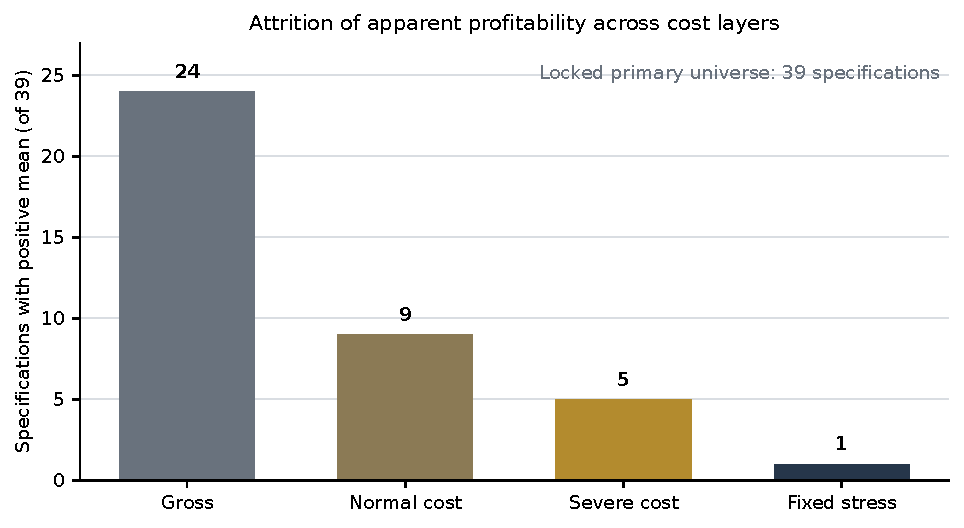
\includegraphics[width=0.86\linewidth]{figure1_cost_attrition.pdf}
\caption{Attrition of positive mean returns across cost assumptions. Bars count specifications, not independent experiments. Source-native normal and severe costs differ by strategy block; fixed stress is the common conservative comparison defined in Table~\ref{tab:costs}.}\label{fig:attrition}
\end{figure}

The attrition is distributed unevenly across source blocks (Table~\ref{tab:block_results}). The successor scan supplied 21,110 rows but only 2 positive severe-cost means. The cross-asset fixed block had 11 of 12 positive gross means, yet none remained positive under severe costs. Event response retained 2 positive severe means, but these were based on very small trade counts. Time-series momentum remained positive under every mean-cost description, whereas the relative-value rule was negative even before severe costs. No source block produced a native pass.

\begin{table}[t]
\centering
\caption{Primary results by source block. Mean basis-point comparisons across blocks are descriptive because horizons and exposure conventions differ.}\label{tab:block_results}
\resizebox{\linewidth}{!}{%
\begin{tabular}{lrrrrrrrrr}
\toprule
Block & Specs. & Rows & Gross $>$0 & Normal $>$0 & Severe $>$0 & Fixed $>$0 & Native pass & Median severe & Best severe \\
\midrule
Successor scan & 19 & 21,110 & 8 & 2 & 2 & 0 & 0 & -4.577 & 2.646 \\
Cross-asset fixed & 12 & 6,584 & 11 & 3 & 0 & 0 & 0 & -4.144 & -2.041 \\
Event response & 6 & 810 & 4 & 3 & 2 & 0 & 0 & -3.734 & 2.007 \\
Canonical TSMOM & 1 & 154 & 1 & 1 & 1 & 1 & 0 & 7.412 & 7.412 \\
Precious-metals RV & 1 & 27 & 0 & 0 & 0 & 0 & 0 & -18.403 & -18.403 \\
\midrule
Total & 39 & 28,685 & 24 & 9 & 5 & 1 & 0 & & \\
\bottomrule
\end{tabular}}
\end{table}

\subsection{Native gates and familywise evidence}\label{subsec:family_results}

None of the 39 primary specifications passed its complete source-native acceptance criteria. Accordingly, none of the 20 families could satisfy the joint support rule. More importantly for scientific rather than commercial interpretation, multiplicity-adjusted evidence was uniformly weak. The smallest family adjusted $p$-value was 0.446 for time-series momentum. The next smallest values were 0.479 for range breakout and 0.565 for volatility expansion. All 20 family decisions were \texttt{NO\_EDGE\_UNDER\_LOCKED\_PROTOCOL}.

Figure~\ref{fig:severe_p} plots each specification's severe-cost mean against its max-$t$ adjusted probability. The five positive severe means are visually separated from the zero-return line, but none is close to the 0.05 threshold. This distinction matters. A rule can have a positive realized mean and still provide weak evidence against a null that accounts for within-family search and dependent returns. Conversely, the absence of a native pass cannot be attributed only to a high commercial CAGR threshold, because the statistical condition independently fails by a wide margin.

\begin{figure}[t]
\centering
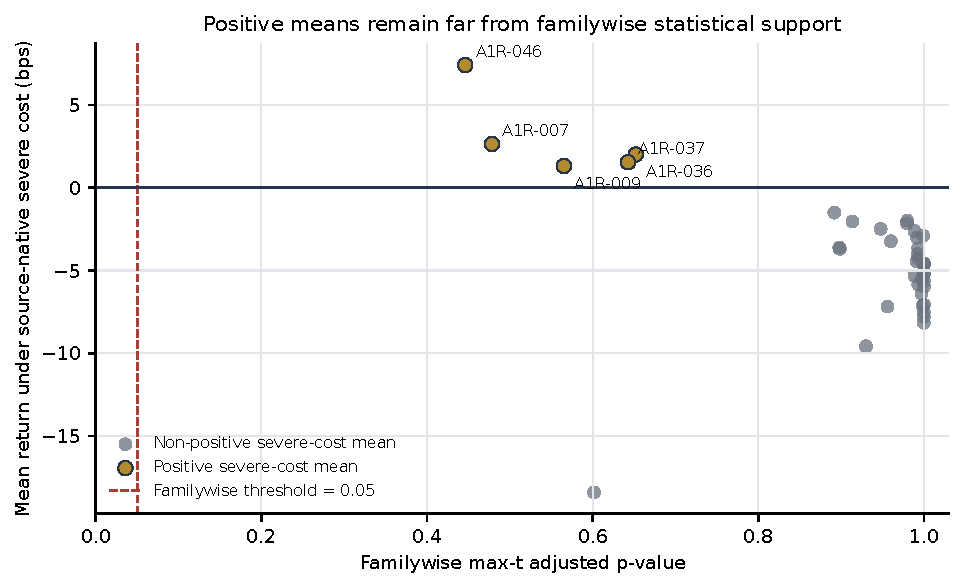
\includegraphics[width=0.88\linewidth]{figure2_severe_mean_vs_family_p.pdf}
\caption{Source-native severe-cost mean and within-family max-$t$ adjusted $p$-value for all 39 primary specifications. Labels identify the five specifications with positive severe-cost means.}\label{fig:severe_p}
\end{figure}

\subsection{Forensic analysis of the five positive severe-cost means}\label{subsec:positive_five}

Table~\ref{tab:positive_five} shows why rank order is not equivalent to support. The largest severe-cost mean belongs to A1R-046, the canonical monthly time-series momentum rule. Across 154 retained monthly observations, its gross, normal-cost, and severe-cost mean returns were 11.644, 9.528, and 7.412 bps. Its severe-cost profit factor was 1.030. Nevertheless, the compounded severe-cost annualized return was -1.53\%, the Sharpe ratio was 0.040, maximum drawdown was 64.3\%, and the mean monthly paired excess over passive volatility-scaled gold was -49.77 bps. Removing the best month left an annualized return of -2.85\%. Only 5 of 13 calendar years were positive and only 1 of 3 chronological folds was positive. A positive arithmetic monthly mean alongside negative compound growth is not contradictory: high dispersion and loss compounding can overwhelm a small average. The adjusted $p$-value was 0.446.

A1R-007, a 48-hour range-breakout rule, produced 2.646 bps under its 4.5-bps severe cost across 455 trades. The profit factor was 1.058, the 10th-percentile block-bootstrap mean was -4.457 bps, and the locked-risk CAGR was 0.18\%, below the 2\% gate. Its fixed-stress mean was -2.854 bps. It also failed cross-feed replication because the severe-cost mean was -0.503 bps on the secondary feed. Thus, the apparently best intraday price-only rule was sensitive both to a modestly more conservative cost and to the price source.

A1R-036 and A1R-037 are short and long 4-hour event-response rules in the gold-lag family. Their severe-cost means were 2.007 and 1.542 bps, but they contained only 12 and 21 trades. Both fell below the 40-trade minimum; both had negative bootstrap lower bounds and became negative after removal of the largest winner. The long rule also concentrated 81.5\% of positive-year profit in one year. Their positive averages are therefore low-information observations rather than reliable event premia.

A1R-009, a volatility-expansion rule, produced 1.313 bps under severe costs across 649 trades. Its profit factor was 1.029, bootstrap lower bound -4.789 bps, and only 40\% of chronological folds were positive. The fixed-stress mean was -4.187 bps. On the secondary feed, the severe-cost mean reversed to -0.406 bps. As with A1R-007, the failure is not one marginal threshold; it is a convergence of cost, resampling, temporal, and feed evidence.

\begin{table}[t]
\centering
\caption{The five specifications with positive severe-cost means. Returns are mean basis points per native trade or rebalance.}\label{tab:positive_five}
\resizebox{\linewidth}{!}{%
\begin{tabular}{llrrrrrrlp{4.4cm}}
\toprule
ID & Family & $N$ & Gross & Severe & Fixed & PF & Adj. $p$ & Cross-feed & Principal failure evidence \\
\midrule
A1R-046 & TSMOM & 154 & 11.644 & 7.412 & 4.591 & 1.030 & 0.446 & Pass & Negative compound return; weak Sharpe; drawdown; passive benchmark \\
A1R-007 & Range breakout & 455 & 7.146 & 2.646 & -2.854 & 1.058 & 0.479 & Fail & Negative bootstrap bound; low CAGR; secondary-feed sign reversal \\
A1R-036 & Event gold lag, short & 12 & 8.007 & 2.007 & -1.993 & 1.103 & 0.652 & N/A & Minimum sample; remove-best-winner and bootstrap failures \\
A1R-037 & Event gold lag, long & 21 & 7.542 & 1.542 & -2.458 & 1.105 & 0.643 & N/A & Minimum sample; instability and year concentration \\
A1R-009 & Volatility expansion & 649 & 5.813 & 1.313 & -4.187 & 1.029 & 0.565 & Fail & Weak PF; negative bootstrap bound; secondary-feed sign reversal \\
\bottomrule
\end{tabular}}
\end{table}

\subsection{Cross-feed replication}\label{subsec:crossfeed_results}

Twenty specifications were eligible for independent-feed evaluation. Thirteen passed all four replication checks and seven failed. Five failures arose because signal Jaccard similarity was below 0.60 even though matched gross-return correlations were high. The remaining two failures were the sign reversals for A1R-007 and A1R-009. Figure~\ref{fig:crossfeed} compares primary and secondary severe-cost means.

\begin{figure}[t]
\centering
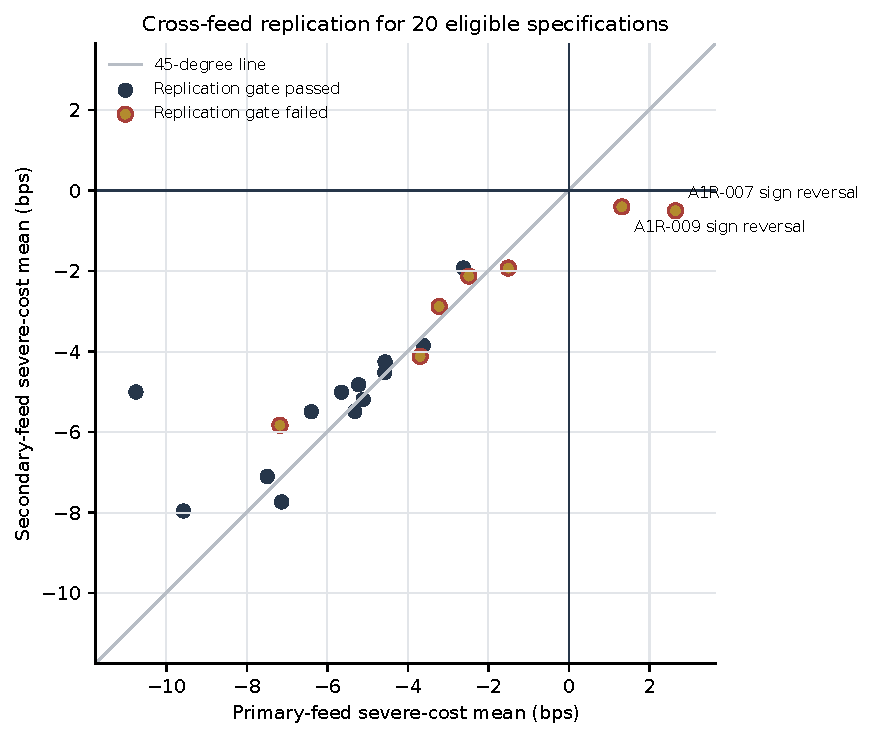
\includegraphics[width=0.77\linewidth]{figure3_cross_feed_replication.pdf}
\caption{Primary- and secondary-feed severe-cost means for the 20 eligible specifications. A gate can fail because of insufficient signal-set overlap even when mean returns lie near the 45-degree line. A1R-007 and A1R-009 fail because the effect direction reverses.}\label{fig:crossfeed}
\end{figure}

The high return correlations among matched trades show that the two feeds generally record similar price changes conditional on a common signal. Jaccard failures reveal a different problem: modest bar-level differences can alter whether a threshold is crossed and therefore which trades exist. This distinction is important for rule-based systems. Outcome agreement conditional on matching events does not guarantee signal reproducibility. A credible trading rule requires both.

Cross-feed non-applicability for 19 specifications is a limitation, not favorable evidence. The cross-asset and event rules require independent reconstruction of the complete feature or event panel, and the relative-value rule requires a second synchronized XAU-XAG pair. The present data contract supports only an independent XAU history for price-only and long-horizon trend rules.

\subsection{Alignment sensitivity, DSR, and PBO}\label{subsec:alignment_results}

The timestamp sensitivity applies to 37 intraday price-derived, cross-asset, and event specifications. Excluding trades overlapping 2019-10-07 through 2019-10-14 caused no severe-cost effect-sign change and no source-native pass-status change. Family max-$t$ rejection and support labels were unchanged. No family was classified as alignment-fragile. This result does not erase the data warning; it demonstrates that the article's decisions are not driven by the diagnosed week.

No specification attained the DSR probability threshold of 0.95. The maximum probability was 0.011284 for A1R-007. Its common-calendar annualized daily Sharpe was 0.155, far below what would be persuasive after 39 eligible trials and non-normal returns. The expected maximum daily Sharpe under the trial count was 0.047736 before higher-moment and sample-size adjustment. DSR therefore reinforces, but does not replace, the native and max-$t$ results.

PBO remains not estimable under the locked protocol. No scalar is reported. Constructing one after seeing the results would require defining a new common performance matrix across incompatible horizons and observation sets, violating the purpose of the lock.

\subsection{Independent audit result}\label{subsec:audit_result}

The independent output-level audit passed with explicit scope limitations. All 16 manifest-listed files were present, and no unlisted run artifact was found beyond the manifest itself. File sizes and SHA-256 digests matched. Primary IDs, family IDs, trade counts, date bounds, and finite-return checks passed. The audit independently reproduced per-specification mean returns and profit factors from 28,685 retained rows, all family max-$t$ statistics and adjusted probabilities, and all DSR outputs. The completed run is therefore internally consistent and statistically reproducible from its retained normalized outcomes.

This audit does not establish that every original source loader, signal, and execution rule would be independently regenerated from raw vendor data by a third party. That stronger claim requires provider access and an end-to-end reconstruction outside the current audit boundary. The replication package is designed to make that boundary visible rather than bury it.

\section{Discussion}\label{sec:discussion}

\subsection{Four layers of evidence attrition}

The results distinguish four failure layers. The first is economic. Gross positivity was common: 24 of 39 specifications. Normal costs removed 15, and severe costs removed 4 more. This pattern indicates that many apparent opportunities were small relative to plausible implementation frictions. Because the normal and severe schedules were source-native, the result is not driven by applying an arbitrary institutional cost to every strategy. The fixed-stress layer then asks a separate question: how many effects have sufficient margin to survive a more conservative common shock? Only the monthly trend mean remained positive.

The second layer is statistical. Five specifications retained positive severe-cost averages, but the smallest max-$t$ adjusted $p$-value was 0.446. These are not near-miss rejections. They are weak familywise evidence. The result directly addresses a possible criticism of the native commercial gates: even if one removed the 1--2\% growth hurdles, no family would satisfy the statistical condition.

The third layer is temporal and structural. Positive event results relied on 12 or 21 trades; the trend rule had unfavorable compounding, fold, year, drawdown, and benchmark evidence; the positive intraday rules had negative bootstrap lower bounds and poor fold behavior. This is what a mean return cannot convey. A sample can have a positive average while most plausible resamples, subperiods, or compounded investment paths remain unattractive.

The fourth layer is measurement reproducibility. Five price-only rules generated materially different signal sets across feeds, and two positive effects changed sign. Threshold strategies are discontinuous functions of their inputs: a small high, low, or close difference can move an observation across a condition and alter the subsequent non-overlap sequence. Cross-feed testing is therefore not merely a price-correlation exercise. It is a replication of the complete decision rule on another measurement system.

\subsection{Implications for gold and international-market research}

The findings are consistent with, but do not subsume, prior precious-metals studies. The negative conclusion for standard or selected intraday strategies parallels the strong attrition reported by \citet{jin2022}. The broader parameter results in \citet{batten2018} demonstrate why multiplicity and persistence must be explicit when a larger rule universe is considered. More recent evidence outside precious metals remains genuinely mixed: selected currency rules can retain predictive content \citep{dockery2023}, whereas very broad equity-market evidence shows decaying predictability, cost sensitivity, and weak persistence of selected rules \citep{rink2023}. The present audit should therefore be read as market- and protocol-specific evidence, not as a vote for one side of a universal technical-analysis debate.

The comparison with recent gold-prediction research requires equal care. Machine-learning studies of price levels, risk premia, and uncertainty-conditioned forecasts address important questions \citep{cohen2023,diaz2023,you2025}, but they do not directly test the estimand reported here. The audit asks whether a fully specified decision rule survives costs, local multiplicity, temporal diagnostics, and a second feed. Its no-go result neither invalidates statistically useful forecasts nor permits forecast accuracy to be treated as evidence of executable profitability. The distinction is especially important when a model has been selected after many feature, architecture, and tuning choices.

The XAUUSD setting also clarifies what cannot be generalized from a broker proxy. The time-series momentum literature typically studies diversified futures and includes return components not represented by a spot-style CFD quote \citep{moskowitz2012,hurst2017}. Failure of A1R-046 does not refute time-series momentum in futures. It shows that this locked 12-month/1-month volatility-scaled implementation did not produce a defensible edge in the available XAUUSD proxy after costs and relative to a passive volatility-scaled gold benchmark. Similarly, a failed gold-silver rule does not reject all cointegration or relative-value models; it rejects one fixed 252-day, $z=2$, next-open implementation.

For international financial markets, the cross-asset block is informative despite its negative result. Most of its 12 gross means were positive, but none survived severe costs. This suggests that a plausible contemporaneous relationship among gold, the dollar, rates, risk assets, energy, and silver is not by itself a tradable lead-lag effect. That interpretation accords with recent evidence that gold's defensive role varies with market, state, and horizon \citep{gurdgiev2024,ryan2024,faraj2025,xu2026}. Economic narrative must be converted into a point-in-time decision rule with enough timing advantage to cover implementation frictions.

\subsection{Research governance and commercially meaningful no-go decisions}

A systematic research program needs a defensible stopping rule. Without one, every failure can be answered by another parameter, filter, asset, or model, and the effective trial count becomes unknowable. The label \texttt{NO\_EDGE\_UNDER\_LOCKED\_PROTOCOL} is therefore a governance decision as well as a statistical description. It closes the tested family under its registered implementation. Reopening it requires genuinely new information: future data not used in the present project, an independently motivated economic mechanism, an independent venue, or a materially different asset universe. Minor retuning on the same period would not be new evidence.

Negative evidence can also support a service-oriented research product. A strategy-audit service should not be evaluated by how often it approves a system. Its value lies in exposing cost sensitivity, search multiplicity, temporal concentration, benchmark dependence, and feed fragility before capital is placed at risk. The present results show that such a system must distinguish descriptive backtest outputs from promotion criteria and must retain an auditable record of every rejected candidate.

The protocol is intentionally fail-closed. Missing cross-feed matches fail the applicable gate; non-applicable tests remain non-applicable; a data-contract failure makes a family untestable rather than negative; and an aborted technical run is separated from an economic rejection. These distinctions prevent operational errors from being rewritten as market findings.

\section{Limitations and scope of inference}\label{sec:limitations}

First, the broader project had seen historical outcomes before the final lock. The consolidated rerun sharply reduces flexibility and prevents result-file reuse, but it does not create a pristine holdout. All probabilities should be interpreted within this registered audit, and the main result is better described as systematic negative evidence than as a classical prospective confirmation.

Second, the independent audit starts from normalized specification-level outcomes. It verifies identities, boundaries, arithmetic, multiplicity, and DSR calculations, but not every raw-data transformation and signal from the original provider files. End-to-end replication requires access to those files and their licenses. The hashes enable exact comparison when authorized copies are available.

Third, the 28,685 retained rows overlap across strategies and time. They cannot be pooled as independent observations. The synchronized bootstrap preserves dependence within each family on a common daily calendar, but residual choices remain, including the 20-day block length and full-sample studentization. Alternative block lengths would be useful robustness checks in a future, separately locked extension. Given that the minimum adjusted $p$-value is 0.446, modest perturbations are unlikely to create a 0.05 result, but that statement is an inference from the margin, not a substitute for a registered sensitivity.

Fourth, source blocks differ in horizon, exposure, cost semantic, and objective. A basis-point mean for a 4-hour event trade is not directly comparable to a monthly volatility-scaled rebalance. Cross-block tables are descriptive, and the primary inferential unit is the economic family under its native contract.

Fifth, cross-feed replication covers only 20 specifications. A complete measurement audit would require independent reconstructions of the cross-asset feature panel, official-event pipeline, and XAU-XAG pair. The absence of such tests neither supports nor rejects those families; their no-go decisions rest on costs, native gates, and multiplicity evidence.

Sixth, XAUUSD is a broker-price proxy. It differs from exchange-traded gold futures in venue, financing, roll, liquidity, and execution. Cost schedules are stress assumptions, not realized fills from a production account. The study authorizes no paper, demo, or live trading and makes no claim about executable capacity.

Seventh, PBO is unavailable by design. The inability to estimate a popular statistic is a limitation, but forcing heterogeneous strategies into an invalid combinatorial matrix would create false precision. The DSR similarly provides only a diagnostic because its common daily calendar differs from source-native evaluation.

Finally, the conclusion is bounded to the registered specifications, source files, reference periods, parameterizations, and gates. It does not establish universal gold-market efficiency, prove that every technical method fails, or rule out future predictability. It establishes that no robust edge was detected in this locked universe under the declared standard.

\section{Conclusion}\label{sec:conclusion}

This paper audits the difference between finding a positive backtest and establishing a defensible trading edge. A locked registry preserved 47 XAUUSD specifications; 39 primary specifications across 20 economic families were recomputed without historical result files and without post-2024 outcomes. The evidence contracted at every layer. Positive means fell from 24 before costs to 9 under normal costs, 5 under severe costs, and 1 under fixed stress. No specification passed its complete source-native gates. No family approached within-family multiplicity-adjusted significance. Seven of 20 eligible rules failed independent-feed replication, including two sign reversals. The timestamp-warning sensitivity changed no decision, and no deflated Sharpe probability approached its threshold.

The null conclusion is deliberately bounded: no robust edge was detected \emph{within the locked universe}. That statement is narrower than declaring the gold market unpredictable and stronger than saying merely that a few chosen strategies lost money. It rests on complete candidate retention, realistic cost layers, search-aware inference, temporal checks, feed replication where feasible, and explicit provenance.

The practical implication is that strategy research should be governed as an evidence-convergence process. Gross profitability is an entry point, not a conclusion. A candidate should advance only when its economic margin, multiplicity-adjusted evidence, temporal behavior, benchmark comparison, and measurement reproducibility tell a coherent story. When they do not, a documented no-go decision is a valid research product. Future work on these families should use genuinely new data or mechanisms rather than reopen the same historical universe after observing its failure.


\section*{Funding}
\FundingStatement

\section*{CRediT authorship contribution statement}
\AuthorName: Conceptualization, Methodology, Software, Validation, Formal analysis, Investigation, Data curation, Writing -- original draft, Writing -- review and editing, Visualization, Project administration.

\section*{Declaration of competing interest}
\InterestStatement

\section*{Data and code availability}
The frozen registry, evaluation protocol, source hashes, normalized specification-level outcomes, derived tables, figure-building code, and independent audit artifacts are supplied with the replication package. The project repository is hosted at \expandafter\url\expandafter{\RepositoryURL}; the immutable repository snapshot referenced in this article is commit \RepositoryCommit. Raw broker and vendor files are not redistributed because their licensing and access conditions may restrict public release. The manuscript reports the immutable SHA-256 bindings needed to verify author-held source files. A qualified researcher may request assistance in reconstructing the permitted inputs, but access to third-party data remains governed by the original providers.

\section*{Declaration of generative AI and AI-assisted technologies in the manuscript preparation process}
During the preparation of this work, the author used OpenAI ChatGPT to assist with manuscript organization, language editing, clarity, consistency checking, and preparation of LaTeX submission files. The author reviewed and edited all assisted content, verified the reported results and cited sources against the research records, retained control over the scientific arguments and interpretations, and takes full responsibility for the content of the published article. AI-assisted code development used during the broader research program is documented in the reproducibility records; all code and outputs used for this article were subject to human review, locked-input checks, deterministic seeds where applicable, automated tests, and an independent output-level audit.

\section*{Acknowledgements}
None.

\bibliographystyle{cas-model2-names}
\bibliography{references}

\end{document}
